To compile this project, follow the steps below:
\begin{enumerate}
    \item Ensure you have a \texttt{C++} compiler installed on your system. Common options include \texttt{g++} (\texttt{std=c++11} or later) and \texttt{clang++}.
    \item Open a terminal and navigate to the directory containing the project's source files.
    \item Use the following command to compile the project:

\begin{verbatim}
cd path/to/project
g++ -o 07 *.cpp
\end{verbatim}

Here, \texttt{07} is the name of the executable file that will be generated.

    \item Run the executable:

\begin{verbatim}
./07.exe
\end{verbatim}

\begin{itemize}
    \item \textbf{Command 1:} Run a sorting algorithm on the user-provided data.
        \begin{itemize}[label=--]
            \item \textbf{Prototype:} \texttt{./07.exe.exe -a [Algorithm] [Input filename] [Output parameter(s)]}
            \item \textbf{Example:} \texttt{./07.exe.exe -a radix-sort input.txt -both}
        \end{itemize}
        
    \item \textbf{Command 2:} Run a sorting algorithm on the data generated automatically with specified size and order.
        \begin{itemize}[label=--]
            \item \textbf{Prototype:} \texttt{./07.exe.exe -a [Algorithm] [Input size] [Input order] [Output parameter(s)]}
            \item \textbf{Example:} \texttt{./07.exe.exe -a selection-sort 50 -rand -time}
        \end{itemize}
    
    \item \textbf{Command 3:} Run a sorting algorithm on ALL data arrangements of a specified size.
        \begin{itemize}[label=--]
            \item \textbf{Prototype:} \texttt{./07.exe.exe -a [Algorithm] [Input size] [Output parameter(s)]}
            \item \textbf{Example:} \texttt{./07.exe.exe -a quick-sort 70000 -comp}
        \end{itemize}

    \item \textbf{Command 4:} Run two sorting algorithms on user-provided data.
        \begin{itemize}[label=--]
            \item \textbf{Prototype:} \texttt{./07.exe.exe -c [Algorithm 1] [Algorithm 2] [Input filename]}
            \item \textbf{Example:} \texttt{./07.exe.exe -c heap-sort merge-sort input.txt}
        \end{itemize}

    \item \textbf{Command 5:} Run two sorting algorithms on the data generated automatically with specified size and order.
        \begin{itemize}[label=--]
            \item \textbf{Prototype:} \texttt{./07.exe.exe -c [Algorithm 1] [Algorithm 2] [Input size] [Input order]}
            \item \textbf{Example:} \texttt{./07.exe.exe -c quick-sort merge-sort 100000 -nsorted}
        \end{itemize}
\end{itemize}

\end{enumerate}

This will compile and link the files \texttt{main.cpp}, \texttt{CommandLine.cpp}, \texttt{DataGenerator.cpp}, \texttt{SortWithCompare.cpp}, and \texttt{SortWithTime.cpp}, along with their corresponding header files.

\begin{figure}[h]
    \centering
    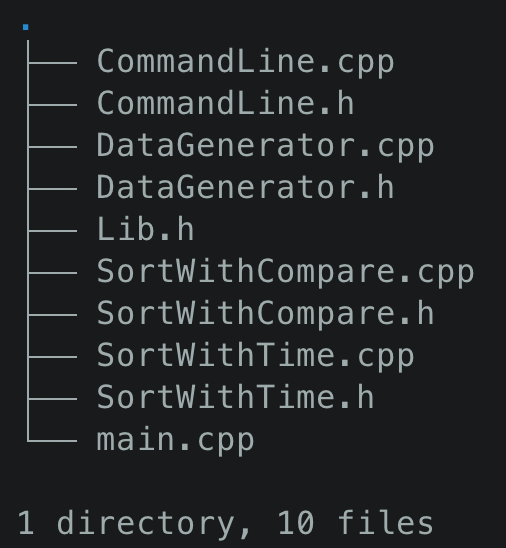
\includegraphics[scale=0.45]{Figures/0. General/tree_folder.png}
    \caption{Folder Tree}
    \label{fig:enter-label}
\end{figure}